\documentclass[•]{article}
\usepackage{pgfplots}

\author{John Niemeyer\\JJNB78@mst.edu}
\title{COMP SCI 5401 FS2017 Assignment 2a}

\begin{document}
\maketitle

\section*{Problem 1: fitness vs Eval graph}
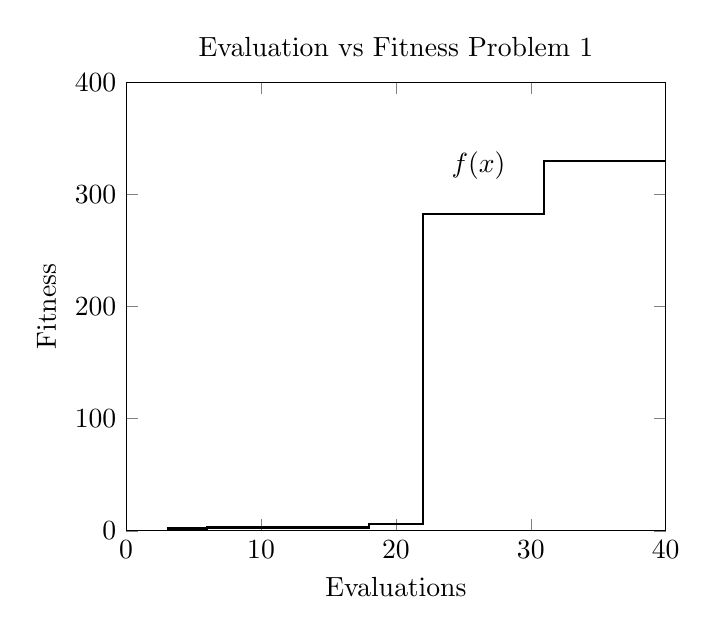
\begin{tikzpicture}
\begin{axis}[
	title = {Evaluation vs Fitness Problem 1},
    xlabel={Evaluations},
    ylabel={Fitness},
    xmin=0, xmax=40,
    ymin=0,ymax=400,
    xtick={0,10,20,30,40},
    ytick={0,100,200,300,400},
    ]
\addplot[const plot, no marks, thick] coordinates {(3,2) (6,3) (18,6) (22,283) (31,330) (40,330)} node[above,pos=.90,black] {$f(x)$};
\end{axis}
\end{tikzpicture}

\section*{Problem 2: fitness vs Eval graph}
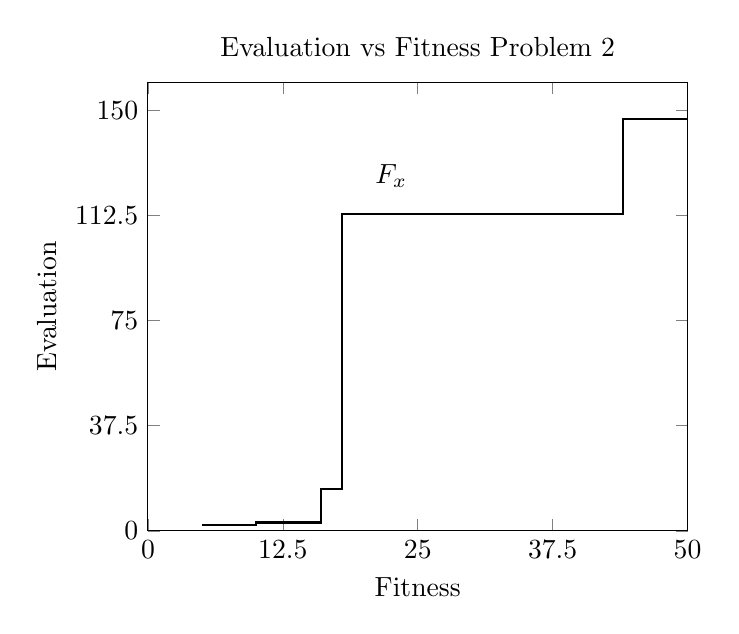
\begin{tikzpicture}
\begin{axis}[
	title = {Evaluation vs Fitness Problem 2},
    xlabel={Fitness},
    ylabel={Evaluation},
    xmin=0, xmax=50,
    ymin=0,ymax=160,
    xtick={0,12.5,25,37.5,50},
    ytick={0,37.5,75,112.5, 150},
    ]
\addplot[const plot, no marks, thick] coordinates {(5,2) (10,3) (16,15) (18,113) (44,147) (50,147)} node[above,pos=.75,black] {$F_x$};
\end{axis}
\end{tikzpicture}

\section*{Problem 3: fitness vs Eval graph}
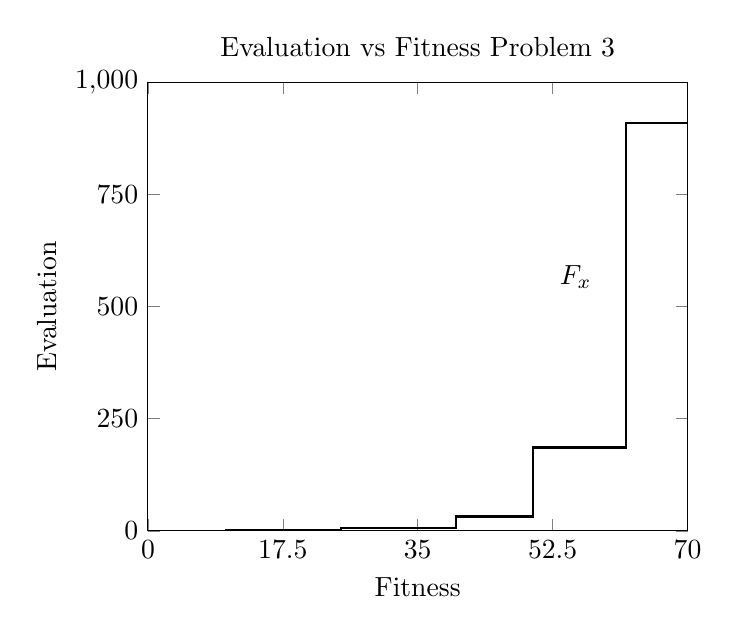
\begin{tikzpicture}
\begin{axis}[
	title = {Evaluation vs Fitness Problem 3},
    xlabel={Fitness},
    ylabel={Evaluation},
    xmin=0, xmax=70,
    ymin=0,ymax=1000,
    xtick={0,17.5,35,52.5,70},
    ytick={0,250,500,750,1000},
    ]
\addplot[const plot, no marks, thick] coordinates {(10,2) (25,6) (40,32) (50,186) (62,910) (70,910)} node[above,pos=.57,black] {$F_x$};
\end{axis}
\end{tikzpicture}
\end{document}